\part{Experimento}
O experimento desenvolvido neste trabalho consiste na criação de um jogo educacional utilizando a tecnologia HTML5. Como tecnologias complementares foram utilizadas: Javascript, CSS3, Queue.js, Highcharts e PhoneGap. O conteúdo educacional escolhido para ser trabalhado no jogo foi expressões algébricas. O jogo consiste em apresentar uma expressão ao jogador e pedir para que ele selecione e resolva cada uma das operações até chegar ao resultado final.

\chapter{Modelo de dados}
Por mais que o experimento não utilize uma aplicação de banco de dados existe um modelo de dados intrínseco expresso no diagrama a seguir.

\begin{figure}[H]
	\caption{\label{gram_cls}Modelo de Dados}
	\begin{center}
	    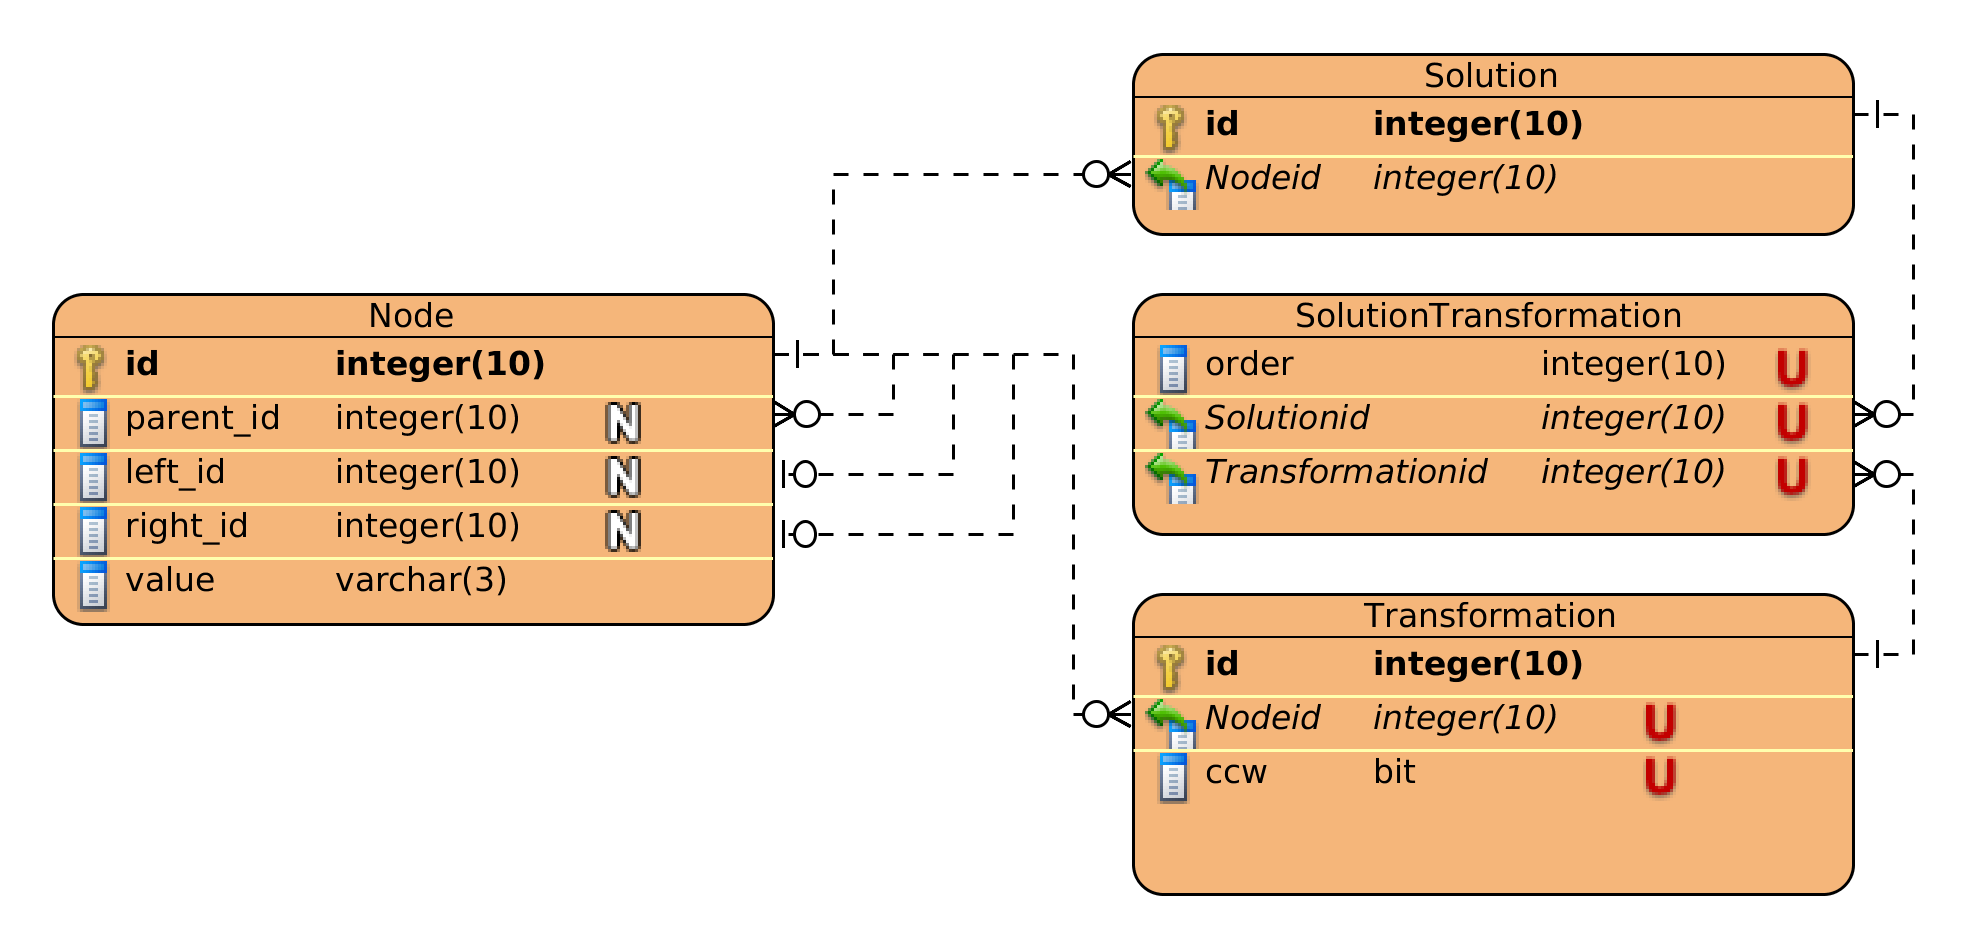
\includegraphics[scale=0.9]{datamodel.png}
	\end{center}
	\legend{Fonte: Produzido pelo autor}
\end{figure}

O diagrama representa as expressões e suas respectivas soluções. Como a estrutura de dados escolhida para representar as expressões foi a árvore, as expressões são armazenadas podem ser armazenadas da mesma forma. Cada nó (Node) aponta para o seu nó pai e seus nós filhos.

As soluções (Solution) para uma determinada expressão são armazenadas na forma de uma lista ordenada de transformações (Transformation). A lista de ordenada de transformações é representada através da entidade SolutionTransformation.

\chapter{Visão geral do fluxo}
O fluxo tem início quando o usuário acessa o jogo – como página de internet ou aplicativo para dispositivo móvel. O jogo inicializa e apresenta o botão “Play” para que o jogador comece os testes. Quando iniciados os testes o jogo escolhe uma expressão e a apresenta ao usuário para que ele selecione uma operação para resolver.

Assim que uma operação é selecionada o programa avalia se esta pode ser resolvida e apresenta a pontuação. Caso a operação selecionada não possa ser resolvida o programa se mantém no estado de seleção, no caso contrário o programa pede a solução para a operação selecionada. Depois que o usuário passa a solução o jogo apresenta a pontuação. Se a solução passada estiver incorreta o jogo permanece no estado de resolução, se a solução estiver correta a aplicação apresenta a expressão resultante.

Enquanto houver operações não resolvidas o fluxo se repete desde a seleção de operação. Quando não houver mais operações a serem resolvidas o programa apresenta os botões “Next...” e “Exit” para o jogador fazer o próximo teste ou sair do jogo respectivamente. Se o jogador for para o próximo teste o fluxo volta para o passo de escolha de expressão, no caso do jogador sair o programa apresenta a tela final.

\section{Inicialização da aplicação}
A função start é responsável pela inicialização da aplicação, recebe como parâmetro o identificador do elemento HTML que irá conter a tela do jogo e insere os principais elementos HTML do jogo, inclusive a tela inicial para que o usuário possa iniciar o jogo.

\section{Escolha da expressão}
A escolha da expressão é feita através da função newXp. Inicialmente a rotina seleciona uma expressão, escolhendo uma das disponibilizadas através do método startDB (executado no início dos testes) ou gerando uma com a função makeExp. Em seguida a expressão selecionada é passada para o contexto do jogo junto de suas soluções.

A criação de novas expressões leva em conta duas variáveis: número de operações e um conjunto de possíveis operações a serem utilizadas. As expressões são criadas de forma aleatória. A probabilidade para cada operação ser sorteada é 1 em n, onde n é o tamanho do conjunto de operações passado. 	Não existe restrição de unicidade para o conjunto de operações que são passadas para a função makeExp possibilitando alterar a probabilidade de que uma determinada operação seja escolhida.

Caso a expressão escolhida tenha sido gerada a fase de passar a expressão para o contexto do jogo envolve a avaliação da expressão para conhecer todas as soluções possíveis para a expressão. A avaliação da expressão é feita através de um algoritmo iterativo implementado na função evaluateTreeIt.

\section{Apresentação da expressão}
A expressão é apresentada utilizando a função appendXp que recebe como parâmetro a expressão e a imprime na tela utilizando a função htmlfy, uma função recursiva que retorna os elementos HTML que representam visualmente a expressão.

\section{Selecão da operação}
A seleção da operação é acionada através de um clique simples com o botão esquerdo do mouse ou toque (no caso de dispositivos móveis) sobre a operação. A função opClick é responsável por tratar tais eventos recebendo como parâmetro o identificador da operação. Internamente a função opClick faz uso da função select que é responsável por avaliar se a operação pode ou não ser resolvida.

\section{Pontuação}
Sempre que houver uma seleção ou tentativa resolver uma operação o jogo avalia se a ação está correta e então apresenta a pontuação através da função spanWarn que recebe como parâmetros o tipo de pontuação, perda ou ganho, e o respectivo valor.

Quando o jogador acerta uma seleção ou resolução na primeira tentavia ele recebe 1 ponto inteiro. Para cada erro o ponto é divido ao meio, assim que se o acerto ocorrer na segunda tentativa o jogador recebe meio ponto. A seleção da última operação não é pontuada por ser uma opção única.

\section{Pedido de solução}
Sempre que uma operação for selecionada corretamente o jogo pede ao usuário a solução através da função askForSolution que apresenta ao usuário a operação isolada seguida de uma caixa de texto, para que o usuário insira a solução daquela operação. Os elementos HTML apresentados contém aqueles retornados pela função htmlfy.

\section{Passagem da solução}
Depois que o usuário inserir a solução na caixa de texto e apertar a tecla ENTER ou tirar o foco da caixa de texto o programa faz uma avaliação da solução passada através da função solSubmit. Caso a solução esteja correta a caixa de texto é transformada em texto simples. Se houver mais de uma possível solução apenas aquela que foi resolvida permanece na tela, as outras são eliminadas da tela.

\section{Exemplo}
O exemplo a seguir exemplifica como o fluxo do jogo é percebido pelo usuário através da interface. Após inicializar a aplicação o usuário vê a tela inicial e o botão “Play”. Após apertar o botão “Play” o jogo apresenta uma expressão para o jogador resolver.

\begin{figure}[H]
	\caption{\label{xp_1} O sistema apresenta a expressão a ser resolvida}
	\begin{center}
	    
\includegraphics[scale=1]{xp_4_1.png}
	\end{center}
	\legend{Fonte: Produzido pelo autor}
\end{figure}

O jogador seleciona uma operação que não pode ser resolvida e perde metade da pontuação da seleção.

\begin{figure}[H]
	\caption{\label{miss_0_5_1}Jogador perde metade da pontuação da seleção}
	\begin{center}
	    
\includegraphics[scale=1]{miss_0_5.png}
	\end{center}
	\legend{Fonte: Produzido pelo autor}
\end{figure}

Em seguida o usuário seleciona a uma operação que pode ser resolvida e ganha a pontuação da seleção.

\begin{figure}[H]
	\caption{\label{score_0_5_1}Jogador ganha a pontuação da seleção}
	\begin{center}
	    
\includegraphics[scale=1]{score_0_5.png}
	\end{center}
	\legend{Fonte: Produzido pelo autor}
\end{figure}

O programa então apresenta a operação isolada e a caixa onde o usuário insere a solução. Este passo será omitido no resto do exemplo.

\begin{figure}[H]
	\caption{\label{xp_2}Programa pede a solução da operação}
	\begin{center}
	    
\includegraphics[scale=1]{xp_4_2_asksol_1.png}
	\end{center}
% 	\legend{Fonte: Produzido pelo autor}
\end{figure}

O jogador erra a solução e perde metade da pontuação da resolução.

\begin{figure}[H]
	\caption{\label{xp_3}O usuário insere um valor errado como solução}
	\begin{center}
	    
\includegraphics[scale=1]{xp_4_3_wrongans_1.png}
	\end{center}
	\legend{Fonte: Produzido pelo autor}
\end{figure}

\begin{figure}[H]
	\caption{\label{miss_0_5_2}O jogador perde metade dos pontos da solução}
	\begin{center}
	    
\includegraphics[scale=1]{miss_0_5.png}
	\end{center}
	\legend{Fonte: Produzido pelo autor}
\end{figure}

Em seguida o valor é corrigido e o usuário ganha a pontuação da solução.

\begin{figure}[H]
	\caption{\label{xp_4}O jogador insere a solução correta}
	\begin{center}
	    
\includegraphics[scale=1]{xp_4_4_rightans_1.png}
	\end{center}
	\legend{Fonte: Produzido pelo autor}
\end{figure}

\begin{figure}[H]
	\caption{\label{score_0_5_2}O sistema pontua o jogador pela solução}
	\begin{center}
	    
\includegraphics[scale=1]{score_0_5.png}
	\end{center}
	\legend{Fonte: Produzido pelo autor}
\end{figure}

O campo de texto é transformado em texto simples e a expressão resultante é apresentada ao usuário. O fluxo seleção/resolução se repete.

\begin{figure}[H]
	\caption{\label{xp_5}O sistema mostra a expressão resultante}
	\begin{center}
	    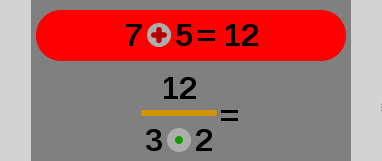
\includegraphics[scale=1]{xp_4_5.png}
	\end{center}
	\legend{Fonte: Produzido pelo autor}
\end{figure}

\begin{figure}[H]
	\caption{\label{score_1_1}O jogador recebe 1 ponto pelo acerto da seleção}
	\begin{center}
	    
\includegraphics[scale=1]{score_1.png}
	\end{center}
	\legend{Fonte: Produzido pelo autor}
\end{figure}

A divisão pode ser resolvida de duas maneiras e o jogo apresenta as duas possibilidades de solução.

\begin{figure}[H]
	\caption{\label{xp_7}O jogo aparesenta duas possibilidades de resolução para a divisão}
	\begin{center}
	    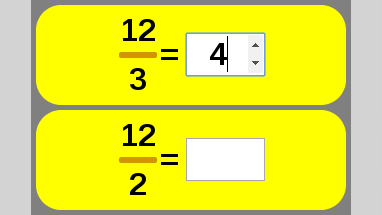
\includegraphics[scale=1]{xp_4_7_rightans_2.png}
	\end{center}
	\legend{Fonte: Produzido pelo autor}
\end{figure}

\begin{figure}[H]
	\caption{\label{score_1_2}O jogador recebe 1 ponto pelo acerto da solução}
	\begin{center}
	    
\includegraphics[scale=1]{score_1.png}
	\end{center}
	\legend{Fonte: Produzido pelo autor}
\end{figure}

O fluxo seleção/resolução se repete.

\begin{figure}[H]
	\caption{\label{xp_8}A nova expressão é apresentada ao usuário}
	\begin{center}
	    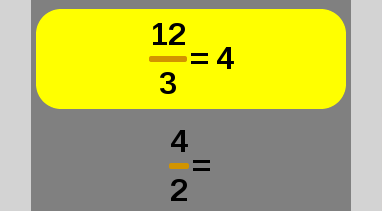
\includegraphics[scale=1]{xp_4_8.png}
	\end{center}
	\legend{Fonte: Produzido pelo autor}
\end{figure}

A seleção da última operação não é pontuada.

\begin{figure}[H]
	\caption{\label{score_0_1}A seleção da última operação não é pontuada}
	\begin{center}
	    
\includegraphics[scale=1]{score_0.png}
	\end{center}
	\legend{Fonte: Produzido pelo autor}
\end{figure}

\begin{figure}[H]
	\caption{\label{xp_10}O jogador insere a última solução a que está correta}
	\begin{center}
	    
\includegraphics[scale=1]{xp_4_10_rightans_3.png}
	\end{center}
	\legend{Fonte: Produzido pelo autor}
\end{figure}

\begin{figure}[H]
	\caption{\label{score_1_3}O jogador recebe a pontuação referente a solução}
	\begin{center}
	    
\includegraphics[scale=1]{score_1.png}
	\end{center}
	\legend{Fonte: Produzido pelo autor}
\end{figure}

	Não existem mais operações para serem resolvidas e as opções de continuar ou sair são apresentadas ao usuário.
	
\begin{figure}[H]
	\caption{\label{xp_11}A tela final é apresentada}
	\begin{center}
	    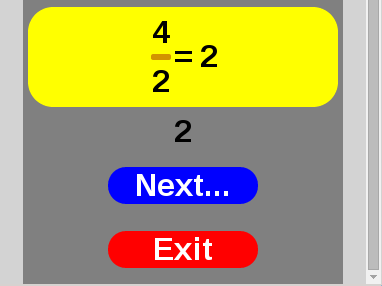
\includegraphics[scale=1]{xp_4_11.png}
	\end{center}
	\legend{Fonte: Produzido pelo autor}
\end{figure}

\chapter{Criação de expressões}

As expressões algébricas utilizadas são linguagens formais pois são um subconjunto de todas as palavras existentes para um determinado alfabeto. Para tanto existe pelo menos uma gramática capaz de gerar a linguagem formal envolvida.

\subsection{A linguagem formal envolvida no jogo}
Vamos partir do conjunto de símbolos terminais que deve conter: as operações de soma, subtração, multiplicação e divisão; um conunto de números dado por um intervalo fechado sobre o conjunto dos inteiros; parênteses. Logo temos T = {+, -, *, /, -2, -1, 0, 1, 2, (, )}. Escolhemos um pequeno intervalo de inteiros neste caso para manter o conjunto pequeno.

	As expressões que fazem da linguagem formal envolvida são do tipo infixa, ou seja, a operação é posicionada no meio de dois elementos que podem ser outras uma outra operação ou um inteiro. Esta escolha se dá por ser o formato que os alunos estão acostumados a ver.
	
\subsubsection{Prefixo, infixo, pósfixo}
Podemos representar uma operação matemática utilizando os três seguintes formatos: prefixo, infixo e pósfixo. No primeiro formato a operação é posicionada em primeiro, antes dos dois operandos. O formato pósfixo é simétrico ao formato anterior, ou seja, a operação é posicionada em último depois dos operandos. Uma vantagem da utilização dos formatos anteriores é a não necessidade de utilizar parênteses para expressar precedência entre as operações. Já no formato infixo a operação é posicionada entre os operandos e necessita utilizar parênteses para expressar precedência entre as operações.

\subsubsection{Parênteses}
A necessidade de utilizar parênteses para expressar precedência entre operações na forma infixa não ocorre para todas as operações na expressão. Os casos são os seguintes: quando uma subtração tem como operando direito outra operação que seja uma soma ou subtração; quando o operando de uma multiplicação ou divisão for uma operação de soma ou subtração; quando um número negativo é operando direito de uma operação.

\subsubsection{Gramática referência}
Tendo em conta os pontos apresentados anteriormente é possível criar uma gramática que seja capaz de gerar as expressões que serão utilizadas no jogo. Algumas simplificações serão feitas a seguir nas produções. Os terminais o e i representam os seguintes conjuntos de terminais respecitvamente o conjunto das operações evolvidas e o conjunto expresso por um intervalo fechado  e contínuo sobre os números inteiros.

	Com a simplificação anterior não existe necessidade de criar uma regra de produção para cada operação e para cada inteiro. Subentende-se que estes terminais, que representam conjuntos, poderiam se desdrobrar em um símbolo não-terminal que produz cada um dos elementos do conjunto que representam sozinho.
	
	A gramática pensada como referência para a solução adotada na criação das expressões é a seguinte:
	
$G: (N, T, P, S)$, onde:

$N = \{S,E\}$,

$T = \{o,i,(,)\}$,

$P$ é o conjunto das seguintes produções:

$S \to (EoE)$

$E \to (EoE) | (i)$,

$\sigma = S$.

Note que a linguagem possui parênteses para todas as operações e inteiros. A linguagem foi pensada assim pois a forma ecolhida para representar suas palavras não foi um texto simples mas sim uma árvore que por natureza já expressa as precedências entre as operações além da necessidade dos parênteses para alguns números inteiros negativos. A lógica de apresentação de parênteses está encapsulada na função htmlfy.

	De acordo com a Classificação de Chomsky, apresentada anteriormente, tal gramática é Livre de Contexto.
	
\subsection{Algoritmo para criação de expressões}
No código Javascript contido no arquivo xpress.js temos a função makeExp responsável pela criação das expressões. A função recebe como parâmetros o número de operações que a expressão deve conter e um conjunto contendo quais operações deversão fazer parte da expressão. A lógica da função makExp está encapsulada em duas funções, makeOps e fillWithInts, onde a primeira gera uma árvore de operações apenas e a segunda preenche a árvore com inteiros, lembrando que a árvore utilizada para representar as expressões é do tipo binária já que cada operação possui dois operandos.

\subsubsection{makeOps}
A função makeOps tem os mesmos parâmetros da função makeExp. Caso as operações não sejam passadas a função utiliza todas as operações (soma, subtração, multiplicação e divisão). A rotina começa com a criação de: uma lista de possíveis operações pai iniciada vazia; uma referência para a raíz da árvore de operações que começa com o valor nulo.

	O passo seguinte é uma iteração sobre o número de operações a serem criadas. Uma operação daquelas passadas como parâmetro é sorteada e passada como parâmetro para a função criadora dos nós que retorna um nó com aquela determinada operação. Se a referência a raíz feita fora da iteração ainda possuir o valor nulo a referência apontará então para o nó criado. No caso contrário o programa sorteia um possível pai da lista, remove da mesma, definindo este como pai do nó criado. 
	
	No final da iteração o programa adiciona novas entradas na lista de possíveis pais. Estas entradas representam a ideia de que o ultimo nó criado pode ser pai a esquerda e pai a direita. Quando não existem mais iterações para acontecer a função retorna o nó referenciado como raíz.
	
\subsubsection{fillWithInts}
No caso de uma árvore incompleta, ou seja, existe pelo menos um operando de uma operação que não foi definido a função fillWithInts pode torná-la completa. A função recebe como parâmetro a raíz da árvore a ser preenchida com inteiros. A função faz uma busca em profundida na árvore para encontrar todas as operações que possuem operandos não definidos e então os define.

	A busca em profundidade é feita utilizando uma pilha de nós a serem analisados. A pilha começa com a raíz que foi passada como parâmetro. Enquanto houver nós na pilha o programa tira o último nó da pilha testando se seus operandos, esquerdo e direito, são nós ou se estão vazios. No caso de o operando ser uma operação o programa o empilha para ser futuramente analisado, se não a rotina cria um nó com um número inteiro e o define como o operando que falta.
	
\subsubsection{Restrição}
Embora o algoritmo criado seja capaz de criar expressões com todas as operações (soma, subtração, multiplicação e divisão) no experimento este é utilizado somente para criar expressões com somas e subtrações, as duas com a mesma probabilidade.

	A restrição foi feita para limitar o escopo deste trabalho pois como requerimento todos os números envolvidos nas expressões, inclusive aqueles que são a solução de uma operação, devem ser inteiros. Neste caso se as expressões possuem divisão o algoritmo na expressão fillWithInts deveria levar tal fato em conta e garantir que os resultados das divisões sejam números inteiros.
	
\chapter{Análise de soluções}
As expressões algébricas envolvidas no experimento podem ter mais de uma forma de solução e para que o jogo possa avaliar corretamente a resolução da expressão feita pelo usuário é necessário fazer a avaliação da expressão a fim de encontrar todas as ordens de resolução possível.

\section{Ambiguidade}
A possibilidade de mais de uma solução para uma mesma expressão se dá pelo fato de que esta expressão pode ser gerada de mais de uma forma utilizando as produções. Por exemplo, 3+4+5 é uma expressão ambigua pois existem duas árvores que podem representá-la:

ARVORE
     
Como vemos a precedência entre as operações varia de uma árvore para a outra. Na primeira a operação 3+4 não tem nenhuma dependência e pode ser resolvida, na segunda isto ocorre com a operação 4+5. A transformação que explica a mudança da primeira árvore para a segunda é uma rotação no sentido horário feita na raíz da árvore. A possibilidade da rotação no sentido horário se dá pois não existe precedência real entre as operações envolvidas significando que as duas podem ser resolvidas no primeiro passo de resolução.

	A rotação utilizada não muda o significado da expressão. Tal fato também ocorre em árvores binárias ordenadas as quais podem ter seus nós rotacionados indeterminadamente sem perder a ordenação de seus elementos. Embora exista tal semelhança as árvores que respresentam as expressões neste experimento não podem ser rotacionadas livremente sem que o significado se altere.
	
	A subtração de uma soma é um caso onde a rotação das operações não pode ocorrer. Por exemplo, 5-(4+3). Existe uma precedência lógica nesta expressão que representa a necessidade de primeiro somar para depois subtrair. A árvore que representa tal expressão é esta:
	
ARVORE
           
A lógica que explica a utilização dos parênteses em operações é a mesma lógica que explica  a possibilidade de rotação na árvore sem perder o significado, ou seja, como a soma é o operando direito da subtração esta deve estar entre parênteses e por sua vez a subtração não pode ser rotacionada no sentido. Além da lógica anterior que explica os parênteses a rotação só pode ocorrer se o nó a ser rotacionado e aquele que toma o seu lugar são operações.

\section{Rotação das árvores}
Como mencionado anteriormente as árvores podem ser rotacionadas tanto no sentido horário como no sentido anti-horário. A lógica que explica a possibilidade de rotação varia entre a rotação horária e a anti-horária já que a consideração que deve ser feita em relação a subtração ocorre apenas quando tentamos fazer uma rotação anti-horária (como no caso anterior da expressão 5-(4+3)).


\subsection{Rotação horária}
	A rotação neste sentido é sempre possível para as operações que possuem como filho esquerdo outra operação, já que a única restrição a ser considerada para saber se a rotação pode ser feita se refere apenas ao filho direito do nó a ser rotacionado.
	
\subsection{Rotação anti-horária}
	A rotação anti-horária não pode ser feita para toda operação que tem como filho direito outra operação, a operação pai em questão não pode ser uma subtração.
	
\section{Números de Catalan}
Como mostrado por Robert Sedgewick e Phillipe Flajolet (2013) os números Catalãos explicam o número de possíveis árvores binárias ordenadas de acordo com o número de nós internos da árvore inicial. O teorema Enumeração de Árvores Binárias enuncia: “O número de árvores binárias com N nós internos e N+1 nós externos é dado pelos números Catalãos” (Robert Sedgewick e Phillipe Flajolet, 2013).

	No caso do experimento algumas rotações não são possíveis nas expressões e sendo assim temos como valor máximo para o tamanho do conjunto das possíveis árvores o número Catalão associado ao número de nós internos na árvore. No entanto se dividirmos as árvores aonde existem as retrições de giro, subtrações com operações como filho direito, podemos encontrar o número de possíveis árvores. Depois de dividir a árvore nos pontos de restrição fazemos a análise para cada árvore resultante e multiplicamos os números para encontrar o número de possíveis árvores.
	
\section{Algoritmo para análise de soluções}
A criação de expressões é um ponto importante no experimento desenvolvido neste tabalho pois evita a necessidade da criação manual de expressões e cria um potencial repositório infinito de expressões. Para tanto é necessário que a aplicação seja capaz de avaliar a expressão criada para encontrar todas as soluções possíveis.

	O algoritmo utilizado para a análise de soluções analisa a árvore que representa a expressão dos nós mais distantes da raíz até os mais próximos. Desta forma cada nó pai conhece todas as transformações possíveis para seus nós filhos. A partir do produto cartesiano de todas as transformações possíveis o nó é testado para rotações sobre todas as transformações contidas no produto cartesiano de soluções dos filhos.
	
	Quando o nó a ser avaliado for raíz o algoritmo testa para conhecer se as soluções avaliadas já existem em um conjunto final de soluções ou não, caso não o algoritmo adiciona tal soluções a este conjunto.
	
	Caso uma nova solução seja encontrada esta é colocada em uma fila para que seja analisada em seguida, assim como a árvore inicial foi. O pseudo-código a seguir explica em mais detalhes o funcionamento do algoritmo para uma dereminada árvore:

\subsection{Desempenho do algoritmo}
Para testar o desempenho do algoritmo de avaliação de expressões a função evaluateTreeItTest foi criada. A função recebe quatro parâmetros de teste. Os dois primeiros são os limites de um intervalo de números inteiro que representam os tamanhos de árvores a serem testadas. O parâmetro seguinte se refere ao número de testes por tamanho de árvore. O ultimo parâmetro é opcional, uma lista de possíveis operações a serem utilizadas na criação das expressões que serão testadas.

	Nos gráficos a seguir podemos observar os resultados dos testes. Os teste foram feitos 10 vezes para árvores de 3 a 9 nós, onde no primeiro teste somente operações de soma foram utilizadas diferente so segundo que também utiliza subtrações.

A diferença nos tempos das séries sem e com soma se devem ao fato de que expressões com subtração tem limitações de rotação. O primeiro gráfico em escala linear mostra o comportamento exponencial da expressão. No gráfico cuja a escala é logarítmica podemos observar com maior clareza como as tempos nas expressões que envolvem subtração variam em um intervalo cujo tempo máximo é o tempo para as árvores que não envolvem subtrações. Isto se deve ao caráter aleatório do algoritmo de geração de expressões. Uma expressão só com somas pode ser gerada mesmo no teste que envolve também subtrações.
